\scanpage{371}
\mspage{95}
du bord du $2$-simplexe

\figure{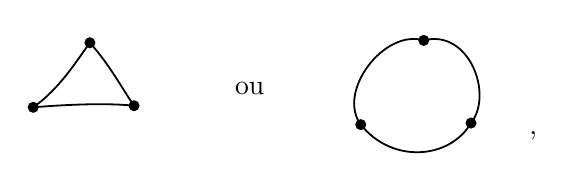
\begin{tikzpicture}[x=1cm,y=1cm,line width=.65pt]
\draw (0,0) .. controls (.34,.24) and (.55,.59) .. (.72,.82) .. controls (.97,.54) and (1.11,.27) .. (1.28,.02) .. controls (.91,.06) and (.36,.03) .. cycle;
\fill (0,0) circle (2pt) (.72,.82) circle (2pt) (1.28,.02) circle (2pt);
\node at (2.75,.24) {ou};
\draw (4.16,-.22) .. controls (3.85,.20) and (4.46,1.00) .. (4.96,.85) .. controls (5.53,1.00) and (5.85,.17) .. (5.56,-.20) .. controls (5.29,-.66) and (4.56,-.72) .. cycle;
\fill (4.16,-.22) circle (2pt) (4.96,.85) circle (2pt) (5.56,-.20) circle (2pt);
\node at (6.35,-.36) {,};
\end{tikzpicture}}

subdivision barycentrique

\figure{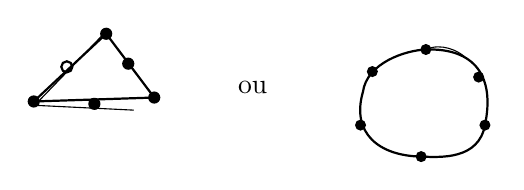
\begin{tikzpicture}[x=1cm,y=1cm,line width=.8pt]
\draw (0,0) -- (.92,.86) -- (1.53,.05) -- cycle;
\draw[thin] (.02,-.04) -- (.88,.85) (.04,-.05) -- (1.27,-.11);
\fill (0,0) circle (2.2pt) (.92,.86) circle (2.2pt) (1.20,.48) circle (2.2pt) (1.53,.05) circle (2.2pt) (.77,-.03) circle (2.2pt);
\draw (.42,.44) circle (2pt);
\node at (2.78,.18) {ou};
\draw (4.18,.12) .. controls (4.23,.49) and (4.72,.65) .. (4.98,.66) .. controls (5.60,.68) and (5.86,.32) .. (5.73,-.30) .. controls (5.65,-.74) and (5.17,-.71) .. (4.92,-.70) .. controls (4.38,-.69) and (4.03,-.40) .. cycle;
\draw[thin] (4.98,.66) .. controls (5.18,.75) and (5.39,.64) .. (5.47,.57);
\fill (4.30,.38) circle (2pt) (4.98,.66) circle (2pt) (5.65,.31) circle (2pt) (5.73,-.30) circle (2pt) (4.92,-.70) circle (2pt) (4.15,-.30) circle (2pt);
\end{tikzpicture}}

(hexagone), que \deleted{\unsure{il n'y}} pour tte application croissante $g:I\to\mathrm{sd}(I)$, sa réalisation topologique est homotope à une application \unsure{constante}, donc $g$ ne peut être un homotopisme dans $\mathrm{Cat}$ (car cela impliquerait que sa réalisation topologique est un homotopisme).

Ceci montre donc que la notion d'homotopisme dans \deleted{\unsure{Hot}} $\mathrm{Cat}$ est \uline{strictement plus fine} que celle pour les réalisations topologiques, ce qui redonne à nouveau substance à l'espoir que l'invariant de Whitehead pourrait \deleted{être} se définir comme invariant d'homotopie'' sur $\mathrm{Cat}$, ou du moins sur une sous-catégorie pleine convenable, telle celle des ens. ordonnés (éventuellement \unsure{restreints} à être finis), ou des maquettes simpliciales. Et même, que \deleted{le}\unsure{l'}\deleted{type d'}\unsure{ens|un} des \inserted{Wh-}types d'homotopie (types d'homotopie simples) peut se
% archive sheet number: 370
